\documentclass[tikz,border=12pt]{standalone}
\usepackage{tikz}
\usetikzlibrary{positioning, arrows.meta}

\begin{document}
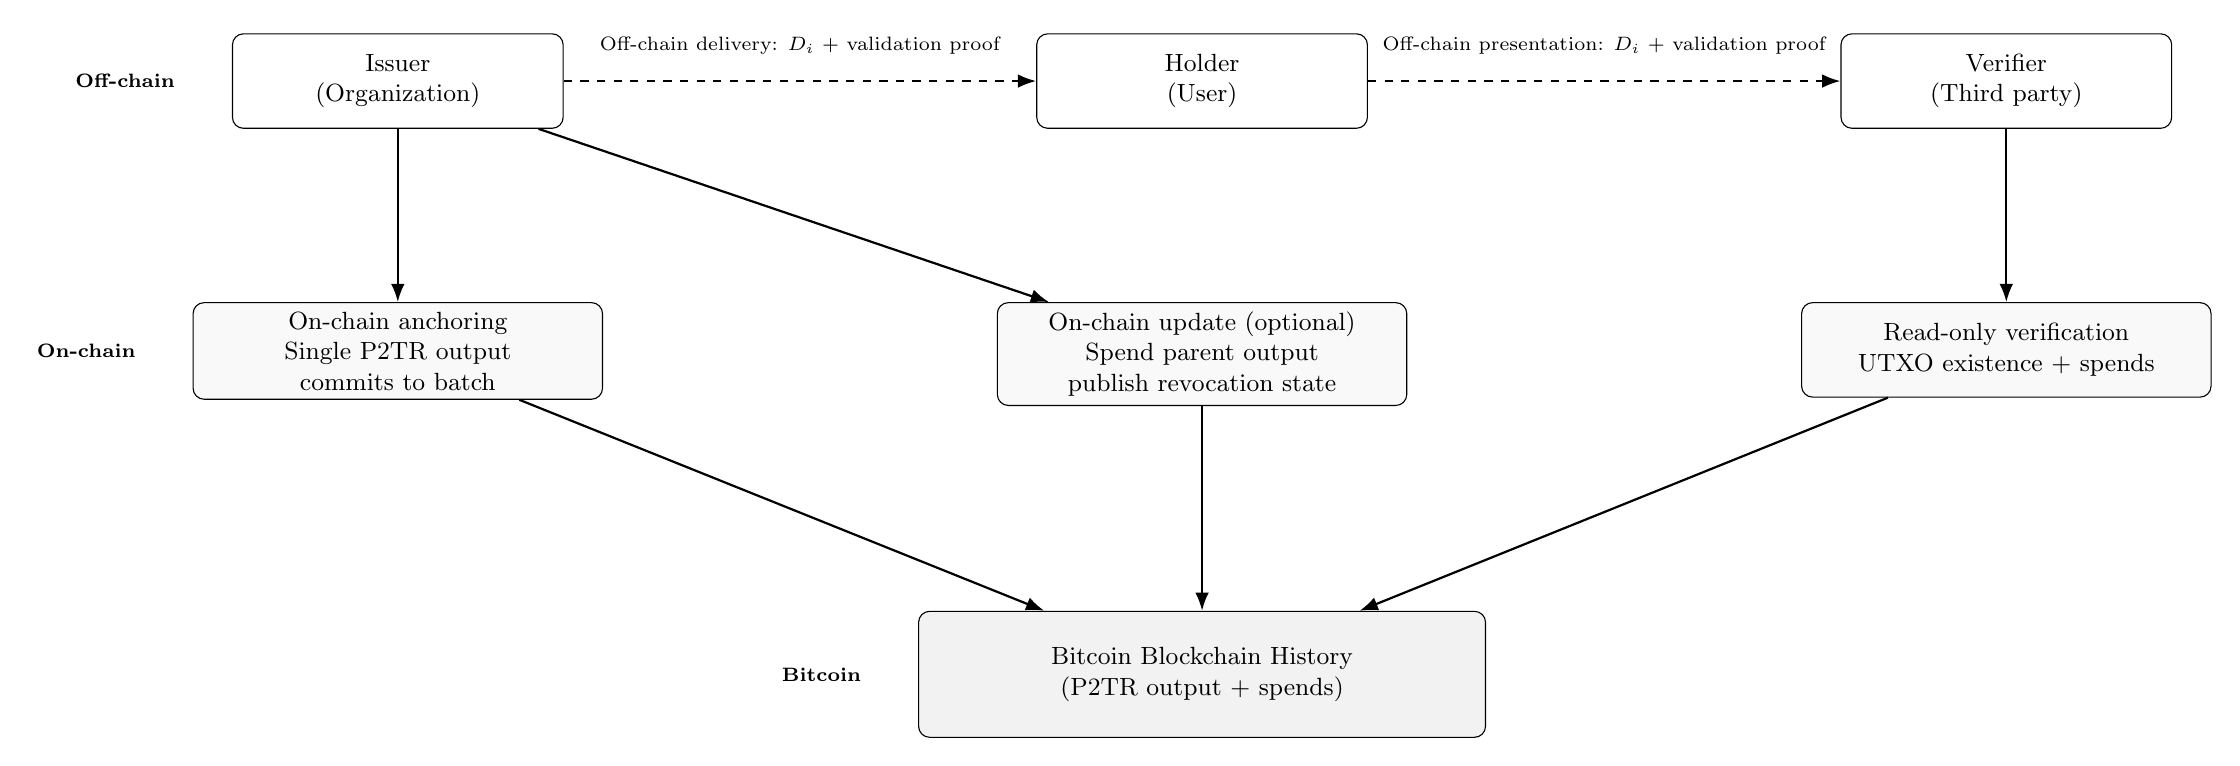
\begin{tikzpicture}[
    font=\small,
    entity/.style={
        draw, rounded corners,
        minimum width=4.2cm, minimum height=1.2cm,
        align=center
    },
    action/.style={
        draw, rounded corners,
        minimum width=5.2cm, minimum height=1.2cm,
        align=center, fill=gray!5
    },
    chain/.style={
        draw, rounded corners,
        minimum width=7.2cm, minimum height=1.6cm,
        align=center, fill=gray!10
    },
    offchain/.style={-Latex, dashed, thick},
    onchain/.style={-Latex, thick}
]

% ===== ROW 1: OFF-CHAIN ENTITIES =====
\node[entity] (issuer) {Issuer\\(Organization)};
\node[entity, right=6cm of issuer] (holder) {Holder\\(User)};
\node[entity, right=6cm of holder] (verifier) {Verifier\\(Third party)};

% ===== ROW 2: ON-CHAIN ACTIONS =====
\node[action, below=2.2cm of issuer] (anchor)
{On-chain anchoring\\Single P2TR output\\commits to batch};

\node[action, below=2.2cm of holder] (revoke)
{On-chain update (optional)\\Spend parent output\\publish revocation state};

\node[action, below=2.2cm of verifier] (read)
{Read-only verification\\UTXO existence + spends};

% ===== ROW 3: BLOCKCHAIN =====
\node[chain, below=2.6cm of revoke] (blockchain)
{Bitcoin Blockchain History\\(P2TR output + spends)};

% ===== OFF-CHAIN FLOWS =====
\draw[offchain] (issuer) -- (holder)
node[midway, above=6pt, font=\scriptsize]
{Off-chain delivery: $D_i$ + validation proof};

\draw[offchain] (holder) -- (verifier)
node[midway, above=6pt, font=\scriptsize]
{Off-chain presentation: $D_i$ + validation proof};

% ===== ON-CHAIN FLOWS =====
\draw[onchain] (issuer) -- (anchor);
\draw[onchain] (issuer) -- (revoke);

\draw[onchain] (anchor) -- (blockchain);
\draw[onchain] (revoke) -- (blockchain);

\draw[onchain] (verifier) -- (read);
\draw[onchain] (read) -- (blockchain);

% ===== LANE LABELS =====
\node[font=\bfseries\scriptsize, left=0.6cm of issuer] {Off-chain};
\node[font=\bfseries\scriptsize, left=0.6cm of anchor] {On-chain};
\node[font=\bfseries\scriptsize, left=0.6cm of blockchain] {Bitcoin};

\end{tikzpicture}
\end{document}
